\section{Ước tính Độ sâu: Nhìn thấy Chiều thứ Ba}
\label{sec:depth_estimation}

\subsection{Giới thiệu: Nghịch lý của Thế giới 3D trong Ảnh 2D}
\label{subsec:depth_intro}

Chúng ta đã học cách mô tả toán học quá trình một cảnh 3D được chiếu thành một ảnh 2D. Trong quá trình chiếu đó, một chiều thông tin bị mất: \textbf{độ sâu} (depth)—khoảng cách từ camera đến từng điểm trong cảnh. Hai cảnh 3D hoàn toàn khác nhau có thể tạo ra cùng một ảnh 2D giống hệt nhau, bởi vì một vật thể nhỏ ở gần và một vật thể lớn ở xa có thể chiếu lên cùng một vùng pixel.

Đây là \textbf{sự mơ hồ hình học cơ bản} của thị giác: không thể phục hồi thế giới 3D từ một bức ảnh 2D đơn lẻ nếu không có thêm thông tin.

Thế nhưng, con người làm điều đó mỗi ngày.

Chúng ta đánh giá được rằng chiếc cốc trước mặt gần hơn chiếc bàn, và chiếc bàn gần hơn bức tường sau. Chúng ta làm điều này bằng cách khai thác hàng loạt các \textbf{manh mối độ sâu (depth cues)} mà bộ não đã học suốt cả cuộc đời: vật thể xa nhìn nhỏ hơn, các đường song song hội tụ về phía đường chân trời, vật thể gần che khuất vật thể xa, ánh sáng và bóng đổ mang thông tin về hình dạng...

\textbf{Ước tính độ sâu (Depth Estimation)} là bài toán trang bị cho máy tính khả năng này: từ một hoặc nhiều ảnh đầu vào, tạo ra một \textbf{bản đồ độ sâu (depth map)}—một ảnh trong đó giá trị mỗi pixel mã hóa khoảng cách từ camera đến điểm tương ứng trong cảnh.

\begin{center}
    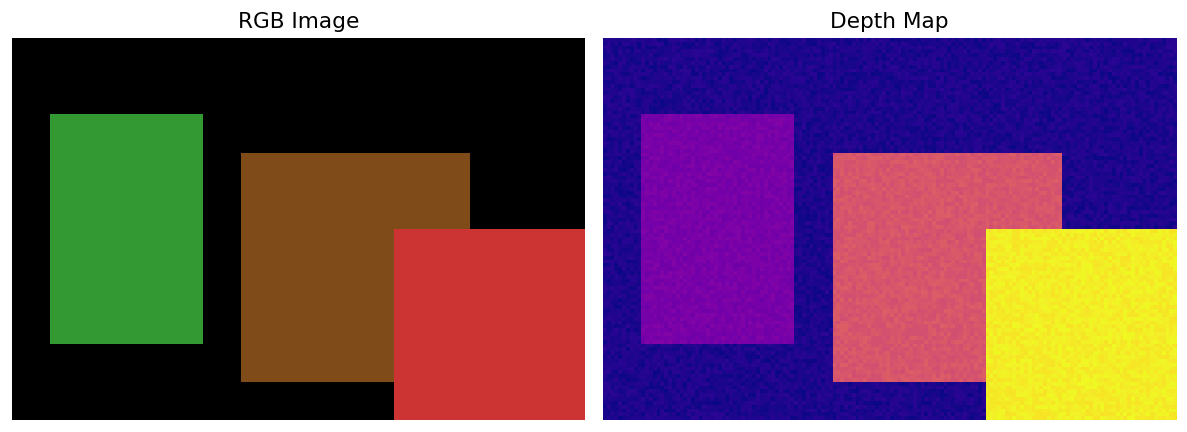
\includegraphics[width=0.9\textwidth]{images/depth_estimation_overview.png}
    \captionof{figure}{Ví dụ về bản đồ độ sâu. (Trái) Ảnh RGB đầu vào. (Phải) Bản đồ độ sâu tương ứng, trong đó các pixel sáng hơn đại diện cho các vật thể gần camera hơn. Bài toán ước tính độ sâu là học cách tạo ra bản đồ bên phải từ ảnh bên trái.}
    \label{fig:depth_map_example}
\end{center}

\subsection{Ước tính Độ sâu bằng Camera Stereo}
\label{subsec:stereo_depth}

\subsubsection{Nguyên lý: Thị sai Hai mắt}
\label{subsubsec:stereo_principle}

Cách tiếp cận cổ điển nhất để đo độ sâu là bắt chước hệ thống thị giác của con người: sử dụng \textbf{hai camera} đặt cách nhau một khoảng gọi là \textbf{baseline} $B$.

Một điểm 3D $P$ sẽ xuất hiện ở các vị trí \textit{khác nhau} trong ảnh của camera trái và camera phải. Sự khác biệt về vị trí pixel ngang này được gọi là \textbf{thị sai (disparity)} $d$. Khi biết disparity, độ sâu $Z$ có thể tính trực tiếp từ hình học stereo:

\begin{equation}
    Z = \frac{f \cdot B}{d}
    \label{eq:stereo_depth}
\end{equation}

trong đó $f$ là tiêu cự của camera (đã biết từ hiệu chỉnh) và $B$ là baseline.

Vật thể \textit{gần} camera có disparity \textit{lớn} (hai ảnh "lệch" nhiều); vật thể \textit{xa} có disparity \textit{nhỏ}. Ở khoảng cách vô cực, disparity tiến về 0.

\subsubsection{Bài toán So khớp Stereo}
\label{subsubsec:stereo_matching}

Vấn đề trung tâm của stereo depth là \textbf{so khớp stereo (stereo matching)}: tìm điểm tương ứng trong hai ảnh, tức là tìm pixel $p_R$ ở ảnh phải tương ứng với pixel $p_L$ đã biết ở ảnh trái.

Nhờ hình học epipolar (đã học ở phần trước), bài toán được đơn giản hóa đáng kể: điểm tương ứng của $p_L$ trong ảnh phải \textit{chắc chắn nằm trên đường epipolar} của $p_L$. Sau khi hiệu chỉnh stereo (rectification), đường epipolar trở thành một đường ngang, nghĩa là ta chỉ cần tìm kiếm $p_R$ \textit{trên cùng hàng} với $p_L$.

Thuật toán cổ điển nổi tiếng nhất là \textbf{Semi-Global Matching (SGM)} \cite{Hirschmuller2008}, kết hợp chi phí so khớp cục bộ với ràng buộc làm mượt toàn cục theo nhiều hướng, cho ra bản đồ disparity chất lượng cao.

Ngày nay, các mạng học sâu như \textbf{PSMNet}, \textbf{RAFT-Stereo} đã thay thế SGM, sử dụng ý tưởng tương tự như RAFT optical flow: xây dựng cost volume 4D và tinh chỉnh lặp.

\subsection{Ước tính Độ sâu Đơn mắt (Monocular Depth Estimation)}
\label{subsec:monocular_depth}

\subsubsection{Từ bài toán thiếu ràng buộc đến học máy}
\label{subsubsec:monocular_motivation}

Stereo depth đòi hỏi hai camera được hiệu chỉnh — một yêu cầu thường không khả thi trong thực tế. Còn nếu chỉ có \textit{một} camera thì sao?

Về mặt hình học thuần túy, bài toán là \textit{ill-posed}: vô số cảnh 3D khác nhau có thể tạo ra cùng một ảnh 2D. Nhưng học sâu đã thay đổi cuộc chơi. Mạng nơ-ron được huấn luyện trên hàng triệu cặp (ảnh RGB, bản đồ độ sâu) có thể \textit{học được} những manh mối ẩn: phối cảnh, kết cấu, bóng đổ, kích thước tương đối của vật thể quen thuộc—và biến những manh mối đó thành ước tính độ sâu.

\subsubsection{MiDaS: Monocular Depth đa miền dữ liệu}
\label{subsubsec:midas}

\textbf{MiDaS} \cite{Ranftl2020} (Mixed Dataset Sampling) là một bước nhảy vọt về tổng quát hóa. Thách thức lớn nhất của monocular depth là mỗi tập dữ liệu (NYU Depth, KITTI, Megadepth...) được thu thập bằng cảm biến khác nhau, có thang đo và phân phối độ sâu hoàn toàn khác nhau.

MiDaS giải quyết bằng cách:
\begin{enumerate}
    \item Huấn luyện trên \textit{nhiều tập dữ liệu đồng thời} với các hàm mất mát affine-invariant (bất biến với phép dịch và tỉ lệ của độ sâu).
    \item Sử dụng backbone mạnh (ban đầu là ResNeXt, sau này là ViT qua DPT).
\end{enumerate}

Kết quả là một mô hình \textit{zero-shot generalization} ấn tượng: hoạt động tốt trên ảnh tùy ý từ internet, không cần fine-tuning.

\subsubsection{Depth Anything: Foundation Model cho Độ sâu}
\label{subsubsec:depth_anything}

\textbf{Depth Anything} \cite{Yang2024} (2024) đẩy xu hướng này lên tầm foundation model. Nó kết hợp:
\begin{itemize}
    \item \textbf{Dữ liệu quy mô lớn:} 1.5 triệu ảnh có nhãn độ sâu cộng với 62 triệu ảnh không có nhãn (unlabeled).
    \item \textbf{Học bán giám sát (Semi-supervised learning):} Dùng một teacher model để tạo pseudo-depth labels cho ảnh không có nhãn, sau đó huấn luyện student model trên cả hai.
    \item \textbf{Encoder mạnh:} DINOv2 làm backbone, đã được pre-train trên quy mô rất lớn.
\end{itemize}

Kết quả: Depth Anything tạo ra bản đồ độ sâu chi tiết và nhất quán đến mức ấn tượng trên \textit{bất kỳ ảnh nào}—từ ảnh chụp trong nhà, ngoài trời, đến ảnh vẽ, ảnh hoạt hình—thể hiện sự tổng quát hóa mà trước đây chưa từng thấy.

\subsection{Ứng dụng và Tầm quan trọng}
\label{subsec:depth_applications}

\begin{center}
    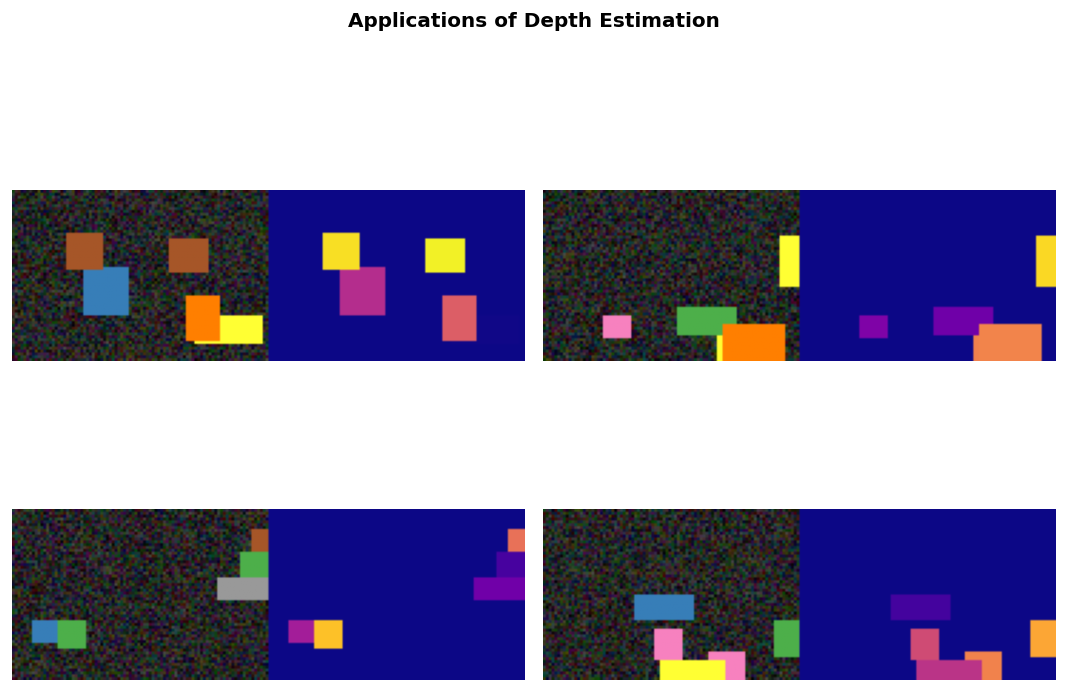
\includegraphics[width=0.85\textwidth]{images/depth_applications.png}
    \captionof{figure}{Ứng dụng của bản đồ độ sâu. (Trên trái) Xe tự lái sử dụng depth map để phát hiện và tránh vật cản. (Trên phải) AR/VR đặt vật thể ảo đúng vị trí trong không gian thực. (Dưới) Robotic grasping — robot cần depth map để tính toán cách cầm nắm đối tượng.}
    \label{fig:depth_applications}
\end{center}

Ước tính độ sâu là nền tảng không thể thiếu của:
\begin{itemize}
    \item \textbf{Xe tự lái:} Phát hiện khoảng cách đến xe phía trước, người đi bộ, chướng ngại vật.
    \item \textbf{Robotics:} Lập kế hoạch chuyển động (motion planning), grasping 3D.
    \item \textbf{AR/VR:} Hiểu cấu trúc 3D của không gian thực để đặt vật thể ảo chính xác.
    \item \textbf{Portrait mode:} Làm mờ nền (bokeh effect) trên điện thoại dựa trên bản đồ độ sâu.
    \item \textbf{3D Reconstruction:} Đầu vào cho các pipeline tái tạo cảnh 3D.
\end{itemize}

\section*{Tài liệu tham khảo}
\begin{itemize}
    \item[1] Hirschmuller, H. Stereo Processing by Semiglobal Matching and Mutual Information. \textit{IEEE TPAMI} \textbf{2008}, \textit{30}(2), 328-341.
    \item[2] Ranftl, R. et al. Towards Robust Monocular Depth Estimation: Mixing Datasets for Zero-shot Cross-dataset Transfer. \textit{IEEE TPAMI} \textbf{2020}.
    \item[3] Yang, L. et al. Depth Anything: Unleashing the Power of Large-Scale Unlabeled Data. In \textit{CVPR}, 2024.
\end{itemize}
